\documentclass[tikz,border=6pt]{standalone}
% Shared visual language for the book's standalone vector figures.
% Keep this file compatible with the TeX Live version used by LyX.
\usepackage{amsmath,amssymb}
\usepackage{array,booktabs}
\usepackage{pgfplots}
\usepackage{pgfplotstable}
\usetikzlibrary{arrows.meta,calc,positioning}
\pgfplotsset{compat=1.17}

\definecolor{BookBlue}{HTML}{0072B2}
\definecolor{BookOrange}{HTML}{D55E00}
\definecolor{BookGreen}{HTML}{009E73}
\definecolor{BookGray}{HTML}{666666}
\definecolor{BookLightGray}{HTML}{D9D9D9}

\pgfplotsset{
  book axis/.style={
    axis line style={black!75,line width=0.55pt},
    tick style={black!75,line width=0.45pt},
    tick label style={font=\small},
    label style={font=\small},
    legend style={
      font=\small,
      draw=none,
      fill=none,
      cells={anchor=west},
    },
    grid style={BookLightGray,line width=0.35pt},
    major grid style={BookLightGray,line width=0.35pt},
  },
}

\begin{document}
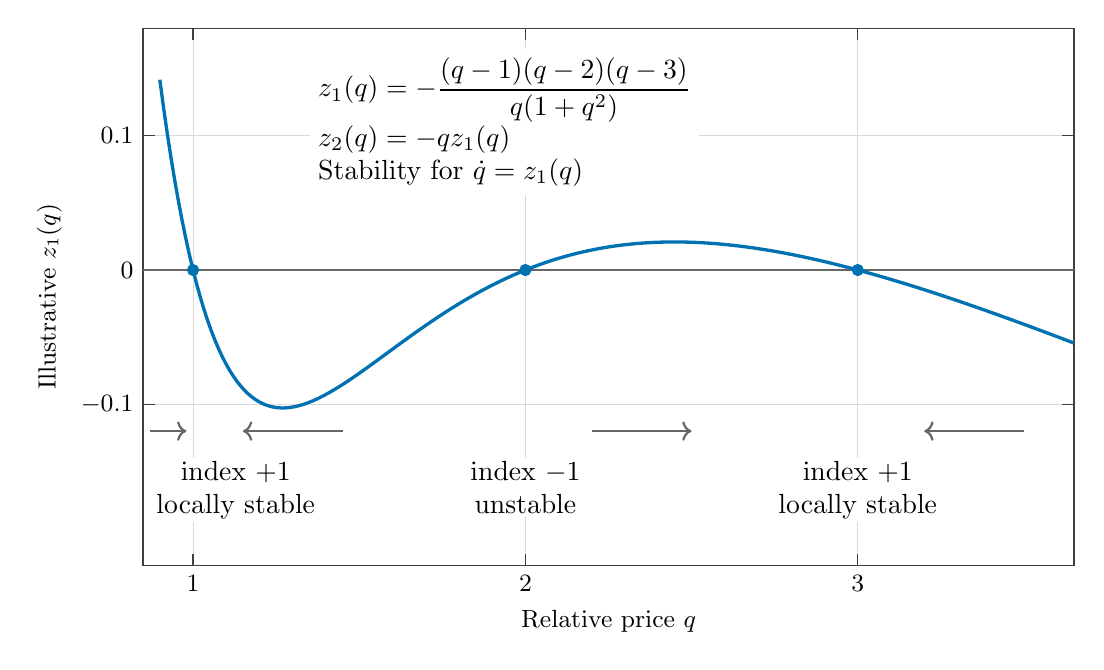
\begin{tikzpicture}
\begin{axis}[book axis,width=13.4cm,height=8.4cm,xmin=.85,xmax=3.65,
 ymin=-.22,ymax=.18,xlabel={Relative price $q$},ylabel={Illustrative $z_1(q)$},
 xtick={1,2,3},ytick={-.1,0,.1},grid=major,clip=false]
 \addplot[black!60,thin,domain=.85:3.65]{0};
 \addplot[BookBlue,very thick,domain=.9:3.65,samples=250]
 {-((x-1)*(x-2)*(x-3))/(x*(1+x^2))};
 \addplot[only marks,mark=*,mark size=2pt,BookBlue] coordinates{(1,0)(2,0)(3,0)};
 \node[anchor=north west,fill=white,inner sep=3pt,align=left] at(axis cs:1.35,.165)
 {$z_1(q)=-\dfrac{(q-1)(q-2)(q-3)}{q(1+q^2)}$\\$z_2(q)=-qz_1(q)$\\
 Stability for $\dot q=z_1(q)$};
 \draw[->,BookGray,thick] (axis cs:.87,-.12)--(axis cs:.98,-.12);
 \draw[->,BookGray,thick] (axis cs:1.45,-.12)--(axis cs:1.15,-.12);
 \draw[->,BookGray,thick] (axis cs:2.2,-.12)--(axis cs:2.5,-.12);
 \draw[->,BookGray,thick] (axis cs:3.5,-.12)--(axis cs:3.2,-.12);
 \node[anchor=north west,fill=white,inner sep=1pt,align=center] at(axis cs:.88,-.14)
 {index $+1$\\locally stable};
 \node[anchor=north,fill=white,inner sep=1pt,align=center] at(axis cs:2,-.14)
 {index $-1$\\unstable};
 \node[anchor=north,fill=white,inner sep=1pt,align=center] at(axis cs:3,-.14)
 {index $+1$\\locally stable};
\end{axis}
\end{tikzpicture}
\end{document}
